\documentclass[a4paper,12pt]{article}
%\usepackage{verbatim}


\usepackage{amssymb}
\usepackage{amsmath}
\usepackage{amsthm}
\usepackage{tikz}
\usepackage{enumerate}
\usepackage{mathrsfs}
\usepackage{graphicx}

\usetikzlibrary{arrows,snakes,backgrounds,positioning,shadows}

\tikzstyle{stan} = [circle,draw=red!50,fill=red!20,thin]

\begin{document}

\title{Control Optimization of Water System for Aeroponics}
\author{Oliver Hennigh \\
Clarkson University}
\renewcommand{\today}{}

\maketitle

\newtheorem*{t1}{Theorem}
\newtheorem*{t3}{Lemma}
\newtheorem*{t2}{Definition}

\begin{abstract}
We have created a model to mimic the behavour of aeroponic water system. Using search algorithms we found optimal or sub optimal control scheme for such systems. The aeroponic water system of investigation uses air compressor to spray fine mists onto free roots of various plants. Optimazation occures for both correct moisture percent in roots as well as compressor active time. We propose our model be used to optimize Clarkson Universities Greenhouse project.
\end{abstract}


\section{Introduction}

In aeroponics nutrient ritch water is spraid onto the free hanging root system of plants. This method of cultivation has many benifits including maximal oxygen intake and high nutrient uptake. The main drawback is the methods need for mist production. It is common that compressors are used to store air preasure and release mists at periodic intervals. This system is used by Clarkson Universities Greenhouse project and has prompted our interest in modeling it. 

The model consist of a compressor, preasure tank, mist pipe and root system. The compressor is activated when the preasure tank drops to a threshold preasure. This causes the compressor to be activated for a precalculated amount of time. The mist pipe switches on and off at a particular frequency and period. The root system is modeld as a drying system with a given max moisture content and linear evaporation rate. ***.

\subsection{Mathematics of Model}
Several assumptions are made about each aspect of the model. There is an assumed linear drying rate of the roots. The mist spray rate is linear dependent on preasure of the tank. The compressor is assumed to increase preasure at a constant rate. Modeling this with equation we get the system


\begin{table}[ht]
\caption{Constants of Interest}
\centering
\begin{tabular} {c c}
\hline\hline
 Variable & explination \\ [0.5ex]
\hline
$P_m$ & air loss rate from mister \\
$W_m$ & water spray rate from mister \\
$E_r$ & evaporation rate of roots \\ 
$M_m$ & max moister content of roots \\ 
$V_t$ & volume of tank \\
$C_r$ & compression rate of compressor \\
$M_c(t)$ & mist control function with values 0 or 1 \\
$P_c(t)$ & pump control function with values 0 or 1 \\
$M(t)$ & moister content of roots in percent \\
$V(t)$ & volume of air compressed in tank \\
\hline
\end{tabular}
\end{table}

\begin{equation}
		  V(t+1) = V(t) + C_r P_c(t) - P_m \frac{V(t)}{V_t} M_c(t)
\end{equation}

\begin{equation}
		  M(t+1) = M(t) + W_m \frac{V(t)}{V_t} M_c(t) - E_r
\end{equation}

\subsection{Optimization}

We wish to optimize both the power usage of the compressor as well as maintaining ideal moister content in the roots. We have included a cost function for the number of times the compressor is activated. This is because starting the compressor often takes several times as much energy as running it. Putting this together gives the following optimization problem.

\begin{table}[ht]
\caption{Optimization constants}
\centering
\begin{tabular} {c c}
\hline\hline
 Variable & explination \\ [0.5ex]
\hline
$I_m$ & Ideal moister content of root \\
$C_s$ & Cost for turning the compressor on \\
$\lambda_r$ & importance factor of root moisture \\
$\lambda_m$ & importance factor of motor usage \\ 
\hline
\end{tabular}
\end{table}

\begin{equation}
		  O = \lambda_r || I_m - M(t) || + \lambda_m || P_c(t) + C_s||
\end{equation}

Because this optimization takes into account both moisture exprestions and cost of running the compressor we have included constants $\lambda_r$ and $\lambda_m$ to control the importance of each componet.


\subsection{Search Space}

The hope for optimizing these equations was to use calculus of variations however there are several real world constrants that make this difficult. Both the mist and pump control must be discrete 0, 1 for relevance to the Clarkson greenhouse project. I believe that the problem can still be solved analyticaly however in the interest of time we have coded the model and simply searched for the optimal solution. Our search space is inspired by the system currently used at Clarkson. 

\begin{table}[ht]
\caption{Search Space}
\centering
\begin{tabular} {c c}
\hline\hline
 Variable & explination \\ [0.5ex]
\hline
$F_m$ & frequency of mister activation \\
$M_t$ & mist activation time \\
$T_p$ & threshold presure to activate compressor \\ 
$C_t$ & compressor activation time \\ 
\hline
\end{tabular}
\end{table}

By randomly trying combinations of these values and running our model on them we could discover the optimal or sub optimal solutions.

\subsection{Appling to Clarkson's Greenhouse project}

Our proposed model is highly dependent on many unknown constants. These values can be found by performing simple experiments and calculations. To illustrate this we have included several instructions on obtaining various constants

\begin{table}[ht]
\caption{Constants cook book}
\centering
\begin{tabular} {p{1 cm} p{9cm}}
\hline\hline
 Variable & method \\ [0.5ex]
\hline
$P_m$ & Measure preasure decrease of tank vs time and do a linear interpilation. Calculated volume change from preasure change \\
$W_m$ & Weight weight increase of root vs time with mist on and do linear interpilation. \\
$E_r$ & Weight root system while drying and do linear interpilation. It should follow a negative exponential. \\ 
$M_m$ & Compare weight of soaked roat and completely dry root. \\ 
\hline
\end{tabular}
\end{table}


\section{Data and Results}

We have coded our model and run several simulations. The following data is the result of the following realistic constant values.


\begin{table}[ht]
\caption{Test Model}
\centering
\begin{tabular} {c c}
\hline\hline
 Variable & value \\ [0.5ex]
\hline
$P_m$ & .3 units per second\\
$W_m$ & .01 percent per second \\
$E_r$ & .0002 percent per second\\ 
$M_m$ & .16 percent \\ 
$V_t$ & 10 units \\
$C_r$ & 2 units \\
$I_m$ & .08 \\
$C_s$ & 3.0 \\
$\lambda_r$ & 3.0 \\
$\lambda_m$ & 1.0 \\ 
\hline
\end{tabular}
\end{table}

By searching on the space described above we obtained and optimal configuration seen bellow. The time period examed was 24 hours.

\begin{table}[ht]
\caption{Optimal Solution}
\centering
\begin{tabular} {c c}
\hline\hline
 Variable & value \\ [0.5ex]
\hline
$F_m$ & 150 seconds \\
$M_t$ & 5 seconds \\
$T_p$ & 3.69 \\ 
$C_t$ & 2 seconds \\ 
\hline
\end{tabular}
\end{table}

These results in them selves are not interesting however they prove that this method works and demonstrates its power.


\section{Produced Data}

If we plot the volume compressed and root moisture content several interesting aspects can be seen. The root graph shows fairly drastic change from 3 percent to 9 percent water content. It can be seen by zooming in on the graph that there are two levels of oscilation pressent. One from the repetitive mist control and the other form

\begin{figure}[ht!]
	\centering
	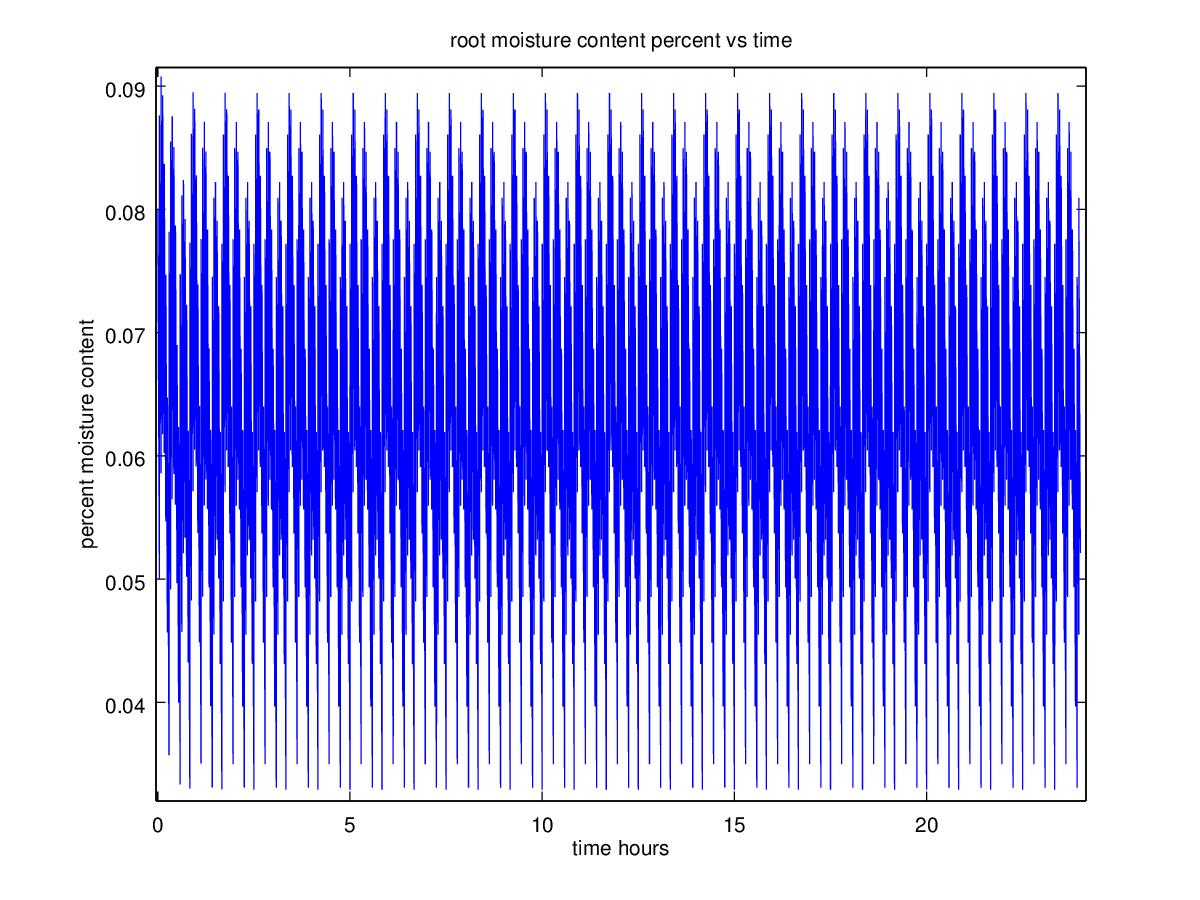
\includegraphics[width=60mm]{root_moisture_content_1.jpg}
	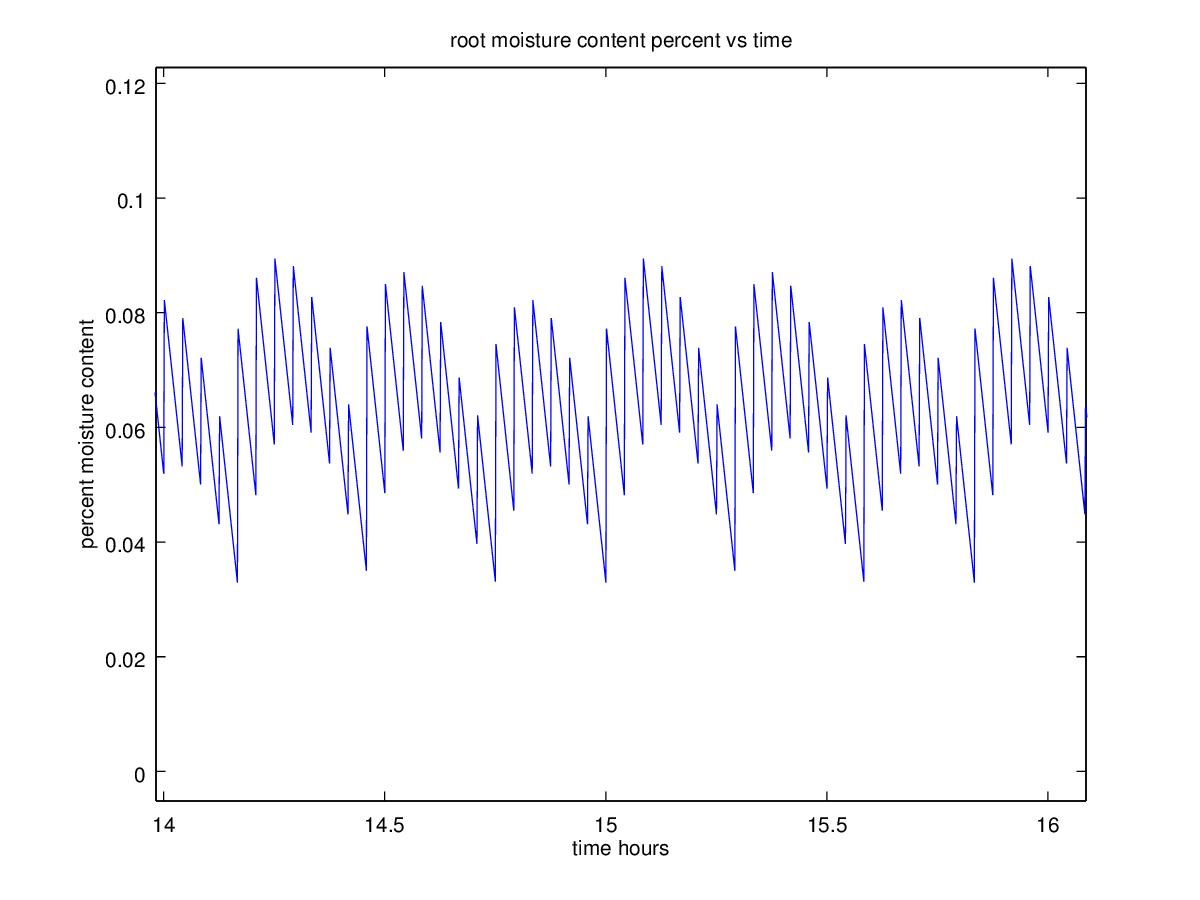
\includegraphics[width=60mm]{root_moisture_content_2.jpg}
	\caption{root moisture content}
\end{figure}

\begin{figure}[ht!]
	\centering
	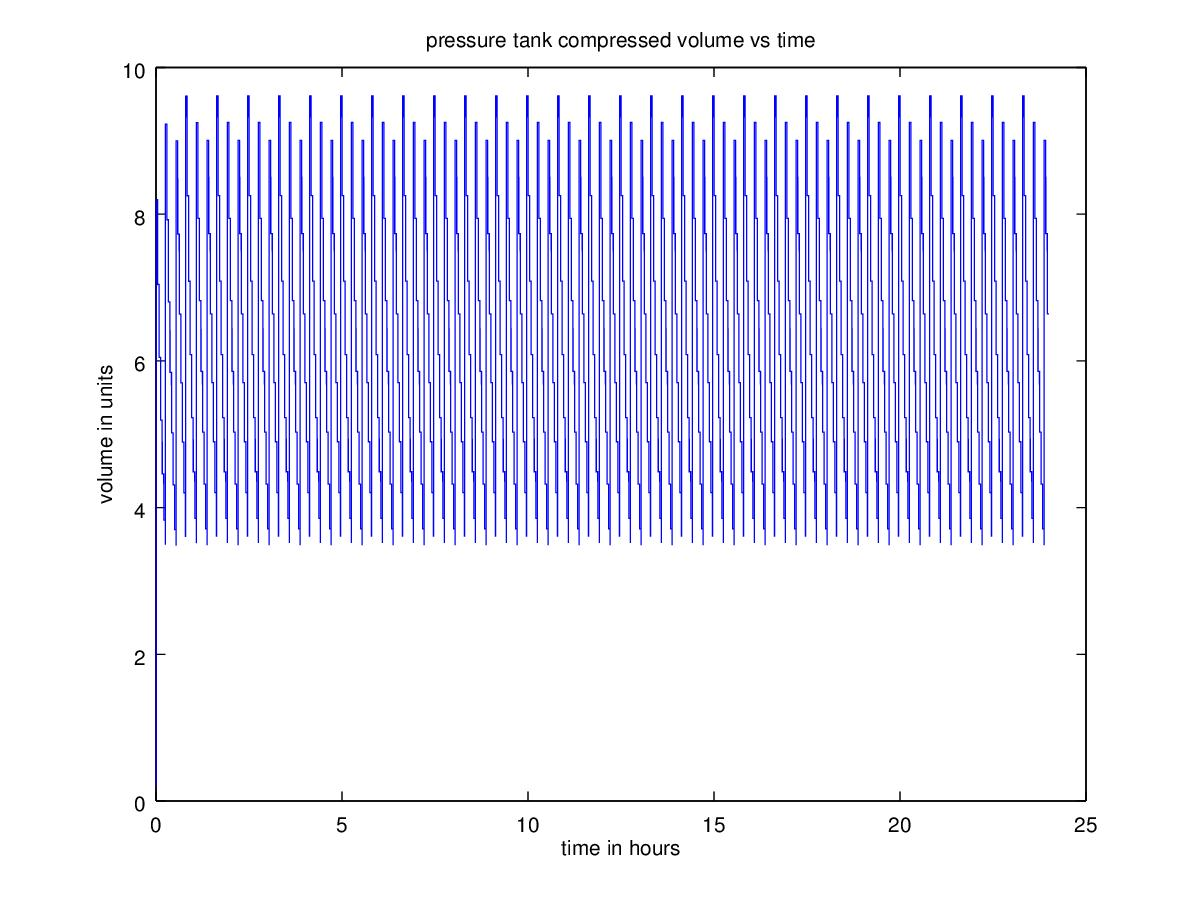
\includegraphics[width=60mm]{pressure_tank_compressed_volume_1.jpg}
	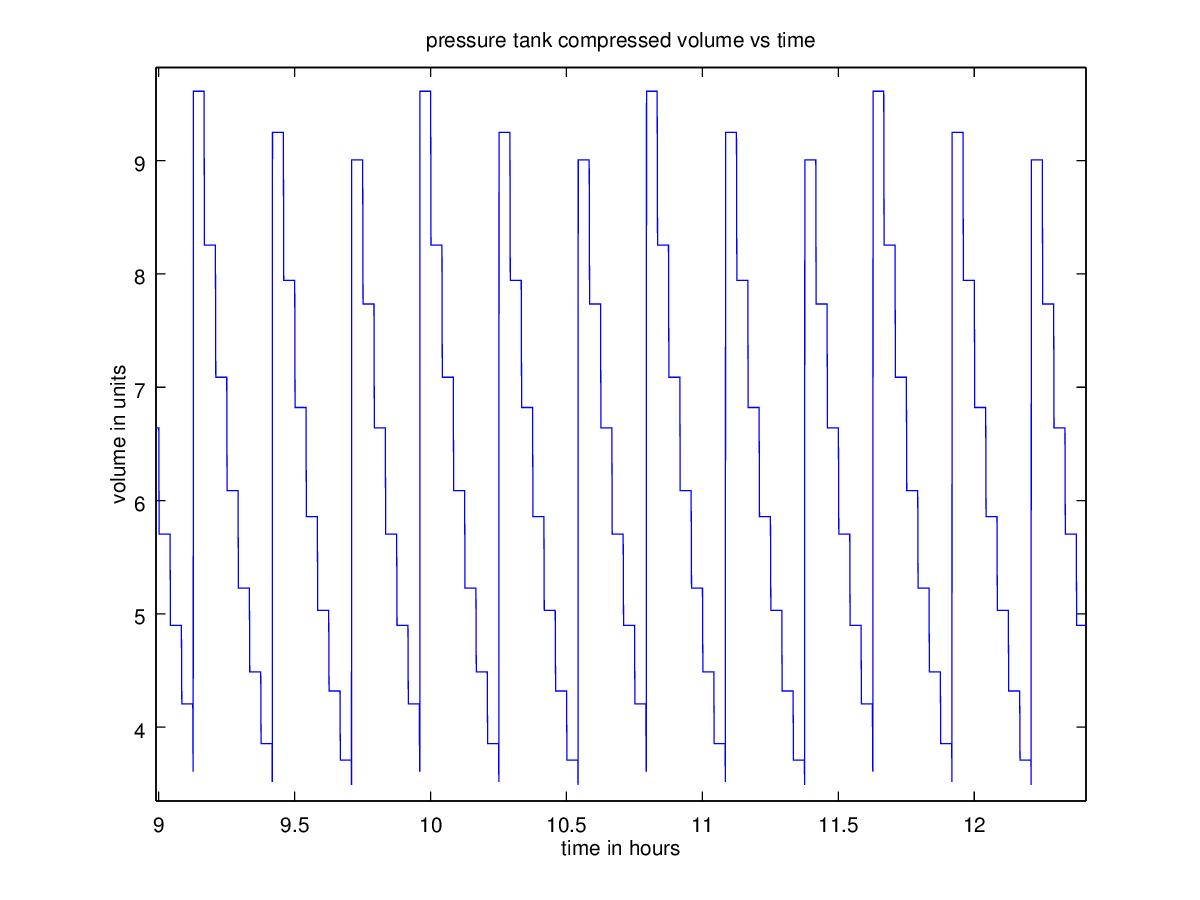
\includegraphics[width=60mm]{pressure_tank_compressed_volume_2.jpg}
	\caption{pressure tank compressed}
\end{figure}




\subsection{Temperature readings over time}


\section{Discussion}


\end{document}
